%!TEX TS-program = xelatex
%!TEX encoding = UTF-8 Unicode

\documentclass[12pt]{article}

\usepackage{algorithm}
\usepackage[noend]{algpseudocode}
\usepackage{amsmath}
\usepackage{amstext}
\usepackage{array}
\usepackage{graphicx}
\usepackage{enumerate}
\usepackage{fontspec}
\usepackage{hyperref}
\usepackage{multicol}
\usepackage[square,sort,comma,numbers]{natbib}
\usepackage{parskip}
\usepackage{url}

\renewcommand{\baselinestretch}{1.2}
\renewcommand{\thesection}{\arabic{section}.}
\renewcommand{\thesubsection}{\thesection\arabic{subsection}}

\newcolumntype{L}{>{$}l<{$}}
\setmainfont{Linux Libertine O}

\makeatletter
\def\old@comma{,}
\catcode`\,=13
\def,{%
  \ifmmode%
    \old@comma\discretionary{}{}{}%
  \else%
    \old@comma%
  \fi%
}
\makeatother

\title{Using Textual Features to Identify Document Reliability}
\author{Julien Cherry \and Patrick McGrath}
\date{April 26\textsuperscript{th}, 2019}

\begin{document}
	\maketitle
	\section{Introduction}

	In early 2018, the American Dialect Society named ``fake news'' its Word of the Year. They note that in 2016, ``its meaning was restricted to fictional or embellished stories presented as authentic news, disseminated for financial gain or for propagandistic purposes'', but that more recently, President Trump has often wielded it ``as a rhetorical bludgeon to disparage any news report that he happened to disagree with'' \cite{ads}. The term’s distinction as the Word of the Year and prevalence in political discourse highlights the seriousness of this issue in the present.

	Given the pervasiveness of fake news and other types of misinformation, people may have difficulty determining the reliability of articles they come across. We approach this problem using supervised learning to assess whether a user can trust a given article online.

	\section{Problem Formulation}

	We formulate the problem by starting with some dataset $D = \{\langle \text{title}_1, \text{author}_1, \text{text}_1, \text{reliability}_1 \rangle \ldots\}$ that consists of a set of tuples, each tuple representing an article. Each article has a title, author, full text, and a reliability judgment. From this dataset, we randomly sample a subset of the articles to get a training set $T_a = randomSample(D)$. Our testing set $T_b = D \setminus T_a$ is the set difference of the original dataset and the training set. We use the training set to train a classifier $C = trainClassifier(T_a)$. And finally, using a novel article $a_n \not\in D = \langle \text{title}_n, \text{author}_n, \text{text}_n \rangle$ (without a reliability judgment), the classifier determines a reliability prediction $p_n \in \{\text{reliable}, \text{unreliable}\} = predict(C, a_n)$ to report whether the article is likely to be reliable.

	\section{Methodology}

	To train our model\footnote{A Jupyter Notebook with our source code is available at \url{https://github.com/PatrickMcGrath29/Trash-Text-Identification/blob/master/classification.ipynb}.}, we used fake news data from data competition platform Kaggle consisting of a 20,800-row CSV dataset for training and a 5,200-row CSV dataset for testing \cite{kaggle}. Each row represents a news article and contains a unique ID as well as the title, author, and text of the article. Additionally, the training file contains a reliability judgment label---1 for potentially unreliable, and 0 for reliable.

	Because we approached the problem with supervised learning and the testing dataset contains no reliability labels, we discarded it. We suspect that the reliability judgments for this dataset are merely unavailable in order to prevent competitors from training on the testing dataset.

	We extracted and cleaned 18,285 articles from the training dataset with the pandas library \cite{pandas}. Here is a random sample of five articles:

	\begin{tabular}{r | p{3cm} | p{2cm} | p{3cm} | l}
		ID & Title & Author & Text & Label \\
		\hline
		191   & Mr. Trump’s Wild Ride - The New York Times        & Robert Draper    & ‘Have you seen the latest polls? I’m beating H... & reliable   \\
		\hline
		7825  & Will Barack Obama delay or suspend the electio... & Michael Snyder   & VIDEOS Will Barack Obama delay or suspend the ... & unreliable \\
		\hline
		17894 & The Man Who Loathed Pajamas - The New York Times  & Jon Caramanica   & Two days before the snowstorm that was suppose... & reliable   \\
		\hline
		17240 & Assange claims ‘crazed’ Clinton campaign tried... & Editor           & Julian Assange has claimed the Hillary Clinton... & unreliable \\
		\hline
		11674 & Rory McIlroy Comes Back Early From Golf Rehab ... & Robert J. Marlow & Rory McIlroy joined President Donald Trump on ... & reliable   \\
	\end{tabular}

	We then randomly withheld 50\% of the articles for use in a testing set. Using scikit-learn \cite{scikit-learn}, we vectorized the data into token--count tuples, building 1,2,3-grams and weighted the features with TF--IDF to prioritize words that are more unique to a given document.

	We then used the data to train each of three classifiers: a naïve Bayes classifier, a stochastic gradient descent classifier, and a Passive--Aggressive classifier. Once the classifiers were trained, we used the model to predict the reliability of articles in the testing dataset.
	
	\begin{figure}
	\caption{This is a graph of the learning curve of the passive aggressive classification algorithm, when using 50\% of the data to train, and the other 50\% to test.}
	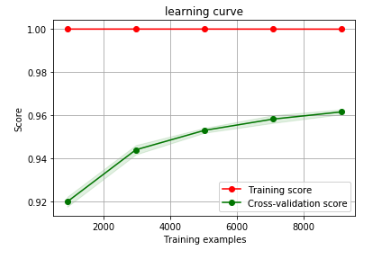
\includegraphics[width=\textwidth]{8k.png}
	\caption{This is the same learning curve, but using 80\% of available data to train.}
	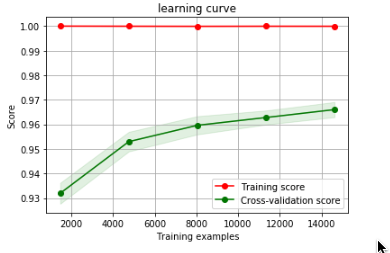
\includegraphics[width=\textwidth]{14k.png}
	\end{figure}
	
	
	\subsection{Passive--Aggressive Classification}

    Passive--Aggressive classification is a process using an online algorithm that works best when streaming data, in that the process uses data to update weights and then discards the data. Similar to other forms of classification, the objective is to classify objects into a series of buckets.

    To do this, we evaluate objects with a series of functions that then determine where in the classification space the object should land. If the classification implies that the weight value (which serves to separate different classification groups) is not correct, then a hinge loss function is used to update the weight.

    The basic algorithm for Passive--Aggressive classification is as follows:

	\def\BState{\State\hskip-\ALG@thistlm}
	\makeatother
	\begin{algorithm}
	\begin{algorithmic}[1]
			\Procedure{Passive--Aggressive Classification}{}
			\State Initialize $w \gets (0, ..., 0)$
			\State Monitor stream...
			\State Ingest new document $d \gets (d_1, ..., d_v)$
			\State Vectorize and apply TF--IDF
			\State Predict classification with $d^T w$
			\State Observe label for document
			\State Compute loss $L \gets max(0, 1 - y d^T w)$
			\State $w_{\text{new}} \gets w + y L d$
			\EndProcedure
		\end{algorithmic}
	\end{algorithm}


	\section{Empirical Results}

	\begin{tabular}{r | l l l}
		                & Naïve Bayes & Stochastic Gradient Descent & Passive--Aggressive \\
		\hline
		accuracy        & 70.67\%     & 94.76\%                     & 96.31\%             \\
		false positives & 2           & 211                         & 150                 \\
		false negatives & 2680        & 268                         & 187                 \\
		specificity     & 33.72\%     & 93.49\%                     & 96.08\%             \\
		precision       & 99.92\%     & 96.67\%                     & 96.12\%             \\
	\end{tabular}

	\textit{Specificity} is calculated as the number of correct negative predictions divided by the total number of negatives.

	\textit{Precision} is the number of correct positive results divided by the number of positive results predicted by the classifier.

	\section{Analysis}

    When beginning the analysis of the findings attained from the three different classification methods we had to reorient ourselves around the objective, which is the identification of misinformation.

    If we defined the optimal approach as the one with the highest precision, that is, the highest accuracy rate when predicting reliable articles, then we would have chosen naïve Bayes as the optimal classifier, given it boasts a precision of 99.92\%. We however thought that the optimal approach would be the one with the highest total accuracy, taking account to the correct classification of reliable and unreliable articles. Passive--Aggressive classification was a clear winner here, with a general accuracy greater than the other two methods.

    After concluding that Passive--Aggressive classification was our optimal approach we began to look at the tokens that had both the highest and lowest weights. These tokens are detailed below.

    \text{Tokens with Lowest Weights}
	\begin{tabular}{r | l l}
		    & Weight        & Token         \\
		\hline
		1   & -10.711168     & said          \\
		2   & -8.084483	    & mr     \\
		3   & -5.679747     & breitbart       \\
		4   & -5.043001	    & twitter          \\
		5   & -4.772107	    & ms        \\
		6   & -4.358110	    & 2017            \\
		7   & -4.255811	    & follow            \\
		8   & -3.650082	    & president         \\
		9   & -3.452179	    & president donald trump     \\
		10  & -3.448971     & president donald           \\
	\end{tabular}

    \text{Tokens with Highest Weights}
	\begin{tabular}{r | l l}
		    & Weight            & Token         \\
		\hline
		1   & 4.908371	        & 2016          \\
		2   & 4.578215		    & us       \\
		3   & 4.427476          & hillary       \\
		4   & 3.794238	        & anti      \\
		5   & 3.779038	        & october           \\
		6   & 3.320482	        & clinton            \\
		7   & 3.044350		        & november          \\
		8   & 2.625362	        & year old            \\
		9   & 2.474821	        & self          \\
		10  & 2.473186          & co         \\
	\end{tabular}

    \subsection{Feature Selection}
    After looking at the token weight pairs that were most influential in determining whether an article was reliable or not, we came to the realization that generally speaking the context of the word is lost with our approach, which decreases our ability to truly identify whether a body of text is misinformation or not. 
    
    Tokens are interpreted individually, with weights then associated to those words, which will then influence the classification outcome of the article. When looking at our initial findings we were concerned about how tokens could appear in both reliable and unreliable articles (independent of any context), perhaps leading to a loss in classification accuracy, and therefore thought that TF-IDF would be an effective tool to reduce the weight of those tokens. This would enable us to focus on tokens that were more indicative of a certain outcome.
    
    When looking at the tables of tokens with highest and lowest weights we noticed that many of the tokens used did not appear to have an inherent association towards reliability or unreliability, and therefore came to the understanding that our classification process here is over-fit to this dataset. Our classification process is attempting to find correlations in tokens that do not likely have an association to the reliability of a corpus of text outside of this dataset. An example of this behavior is demonstrated in the table listing tokens with the highest weights. The token \textit{2016} has a high association to reliability, however it is not reasonable to assume that articles that refer to the date 2016 are as an absolute more reliable than those that do not.

    \subsection{Bias}
    
    When analyzing the results of the classification we identified clear political bias in the outcome. Tokens include \textit{clinton} and \textit{hillary} have high weights, meaning they are more more indicative of an article being reliable. Tokens like \textit{donald trump} and \textit{president} on the other hand have low weights, indicating an association towards unreliability. This political bias is likely a result of the articles that are included in the dataset, indicating that there are likely more reliable articles with a mention of Hillary Clinton in it than there are articles with a mention of Donald Trump.
    
    \subsection{Machine Learning vs. Human Classification}
    
    When using Passive Aggressive classification we had a total of 150 false positives. These articles are labeled as reliable but predicted as unreliable by the classifier. We spent some time looking into these false positives, to see if we would be able to identify whether an article was reliable or unreliable without knowing what the datasets label was.
    
    This is a passage from one of those articles, \textit{Failed presidential candidate Hillary Clinton allegedly spent ‚tens of millions of dollars‚ on digital youth outreach during her campaign, reportedly spending an extra \$30 million on internet adverts}. When we were looking at this article we assumed that it was unreliable, given the biased informal phrasing at the beginning of the sentence. The Kaggle dataset however has this article labeled as reliable. Either this article was labeled incorrectly, or the creators of this dataset operate with a slightly different definition of what reliability and misinformation is. Given that we were unable to accurately classify this document correctly according to the provided label, it is understandable that the passive aggressive classifier was also not able to classify it.

	\section{Future Work}

	Naturally, we would like to improve the accuracy of our model. One way we could do this is to further investigate what kinds of articles are misclassified, which would allow us to deduce one or more underlying factors that causes certain misclassifications, which we could then correct for. Another way we could improve our model would be to improve context around words. At the moment our method only takes into account 1,2,3-grams. We think if we were to use Word2Vec or Doc2Vec to preserve the context around words then we would be able to have better representations of how words are used, and establish a more accurate classification for whether something is misinformation or not.

	Depending on the use case, it would also be wise to tweak the specificity and precision of the classifier. We could, for example, decide that false negatives are better than false positives in a particular use case.

	Practically speaking, work in this area could be used to inform social media users whether linked articles are likely to be reliable or not. However, its implementation need be informed---Pennycook et al. found that labelling disputed articles with a warning causes unlabelled articles to appear more accurate. Crucially, they found that this \textit{Implied Truth Effect} is reversed when verified articles are also labelled \cite{pennycook}.

	\section{Reflection}

	When considering what project we should work on we came together around common interests in machine learning, and hoped to see how it could better inform people about the quality of content that they were reading. We spent the first several milestones learning about different machine learning practices and approaches, and ended up working towards a series of goals that we thought would be manageable given the constraints of this project. 
	
	In retrospect, we think it would have been beneficial to have a more specific definition for what misinformation is, so that we would better be able to measure our approach against this goal. Our current definition is closely associated to a specific dataset, and what that dataset determines is reliable and not reliable, and so our current goals are measured against the findings for this dataset, instead of a broader definition of what misinformation actually is.
	
    An ideal definition for misinformation as it relates to the scope of this project would need to be very specific, and would take into account a series of different factors that would collectively indicate whether something is misinformation or not. This set of factors could include political bias, percentage of factual content, etc...

	\bibliographystyle{plainnat}
	\bibliography{references}
\end{document}
